% !TEX root = ../main.tex
\chapter{Train the Deep Model for Prediction}\label{ch:chapter4} % For referencing the chapter elsewhere, use \ref{Chapter1}
%
%%----------------------------------------------------------------------------------------
The convolutional neural networks (CNNs) consist of neurons that have 
weights and bias, which can be trained using large datasets for solving 
computer vision tasks.
In this chapter, our architecture of
deep convolutional neural network for intra mode prediction 
is illustrated.
Then the hyper-parameters of our deep model is introduced
with explanations.
At the end of the chapter, the stopping criteria and training results 
are presented.
\begin{figure}
    \centering
    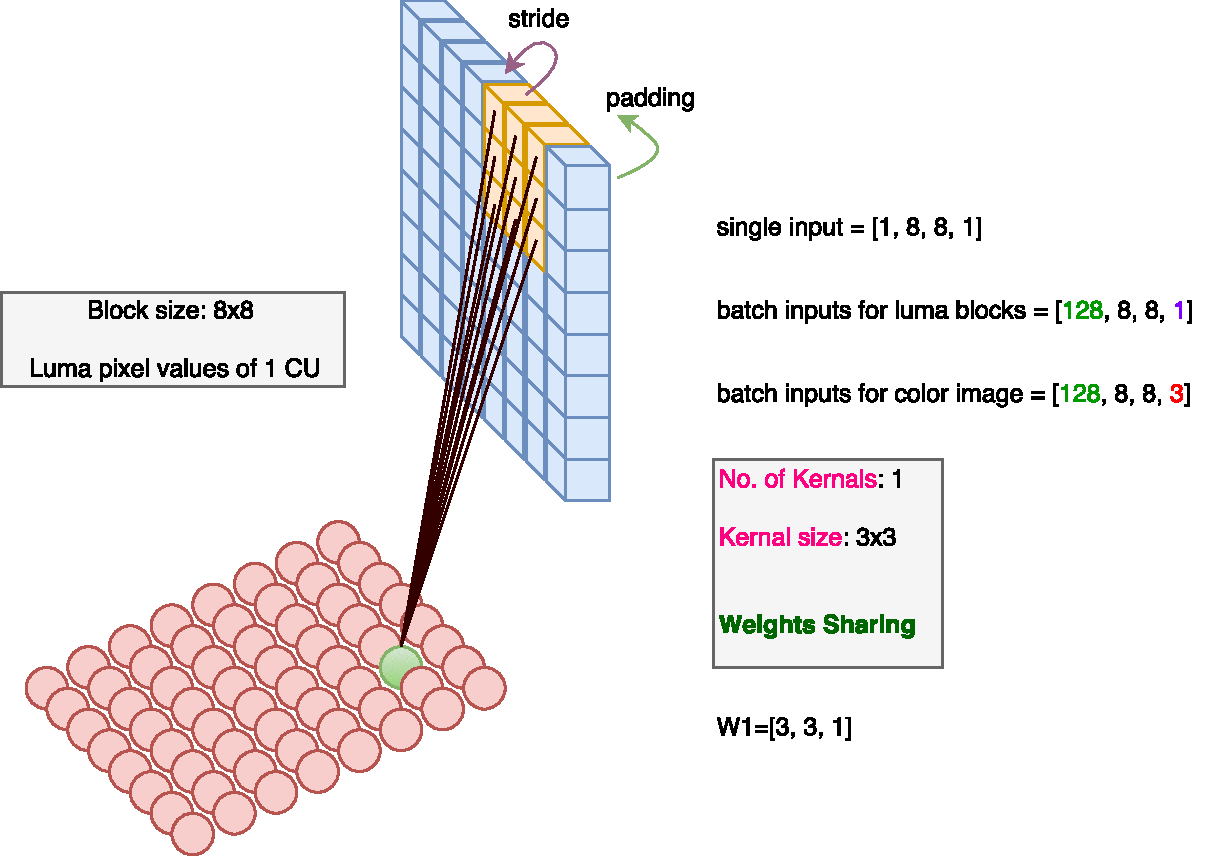
\includegraphics[width=\textwidth,height=\textheight,keepaspectratio]{Figures/cnn_illustration.pdf}
    \caption[Two types of the residual units]{
        Two types of the residual units.}\label{fig:cnn-illustration}
\end{figure}

\section{The Architecture of CNN}\label{sec:cnn}
There exist many kinds of convolutional neural networks while the 
major difference that distinguish them from each other
is the uniqueness of each architecure.
Figure~\ref{fig:cnn-illustration} on 
page~\pageref{fig:cnn-illustration}
illustrates the basic architecture
of the convolutional neural networks.
The light blue cubics represent the Luma pixel values from a single
coding unit (CU) of size \(8\times8\) while the yellow cubics
shows a kernel of size \(3\times3\) that slides over the
CU in both directions.
At each position, the kernel does a weighted sum of all its inputs,
then adds biases. The output from the
region it covers will be fed into a neuron right 
below the covered region.
Although both are artificial neural networks, 
the big difference between multilayer perceptron and 
CNN is that weights of the neurons are shared in the latter case.
For example, all the neurons in Figure~\ref{fig:cnn-illustration} on
page~\pageref{fig:cnn-illustration} are reusing the same patch of
parameters, i.e., weights and biases.
For a single kernal of size \(3\times3\), it has 9 weights.
Apparently this amount of learnable parameters is just not enough.
More degrees of freedom are needed to enable 
the learning capability of a neural network.
For this reason, multiple kernels will be used instead of one single kernal.
If many kernels are stacked in a convolutional neural network such that
the architecture looks very deep, the network is called deep neural network
instead of simply neural network which typically refers to shallow ones.
In the deep convolutional neural networks, it can be imagined that
each convolutional layer comprising multiple kernels which subsequently produces
a three dimensional volume of the outputs.
After the convolutional layer, there normally exist activating layer where
the specified activation function will be applied to each single output
inside the output volume from the convolutional layer.
Followed by the activating layer, there is a pooling layer.
In the previous years, the maximum pooling and average pooling 
are popular methods for reducing the dimension of the outputs
from convolutional layers.
Nowadays, instead of applying a conventional pooling, 
a convolutional layer of larger stride is utilized.
Such a combination of convolution-activation-pooling will
be replicated multiple times for a single convolutional neural network.
In the tail of the network, a fully-connected layer can be used
to compute the probability of each target class for the 
classification problems.

Our network is exactly built from the above description except the 
fact that we have adopted the identity mapping 
\(h(\mathbf{x}_l)=\mathbf{x}_l\) in the Residual 
Neural Network from~\parencite{RN67}.
It has been shown in~\parencite{RN68} that
the identity mapping in the residual units
can enable the direct propagation of information
from one layer to any other layers.
Such a nice property brings vital benefits
for deep neural networks such that the accuracy
saturation problem can be alleviated.
As a result, ultra-deep models are able to
learn desired representations for solving
problems.
Besides, with the identity mapping, the network
is able to converge faster hence the training time
required for a deep model can be reduced.
% The architecture of the deep 
Figure~\ref{fig:basic-resnet-structure} on 
page~\pageref{fig:basic-resnet-structure}
shows two types
of the residual units which implement the identity mapping
via shortcut connections from the beginning of the block
to the end of the same block.
\begin{figure}
    \centering
    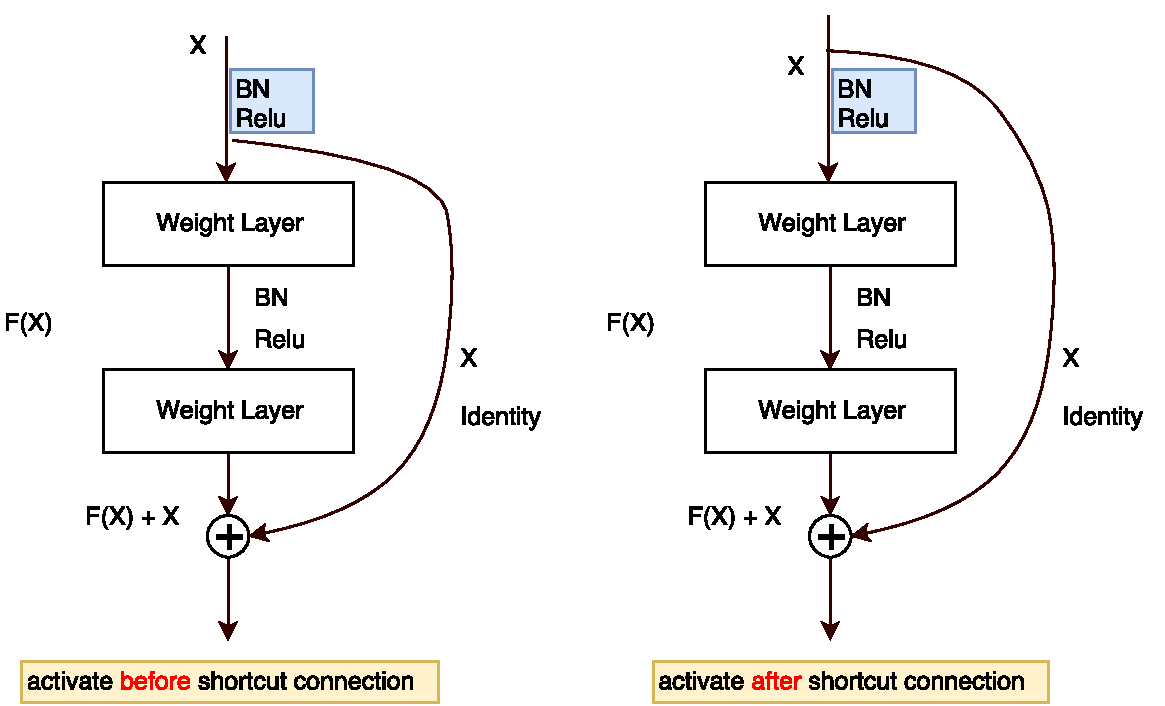
\includegraphics[width=\textwidth,height=\textheight,keepaspectratio]{Figures/basic-resnet-structure.pdf}
    \caption[Two types of the residual units]{
        Two types of the residual units are shown here.
        BN stands for Batch Normalization while
        Relu stands for Rectified Linear Unit.
        }\label{fig:basic-resnet-structure}
\end{figure}

The architecture of the deep convolutional neural 
network used for intra mode prediction in our work
is shown in Figure~\ref{fig:our-architecture} on
page~\pageref{fig:our-architecture}.
The first layer consists of 16 kernels where
the receptive fields are 
simply stacked on top of each other.
In the middle of the network, there are
three variants of resnet unit, each unit
is duplicated five times to deepen the network
for more learning capacities.
Batch Normalization is employed to regularize
the data inputs as well as the outputs from each layer.
The activation function is the most popular one named Relu.
In the end of the convolutional layers, global average pooling
has been performed before the fully-connected layer which 
tells the prediction results.


\begin{figure}
    \centering
    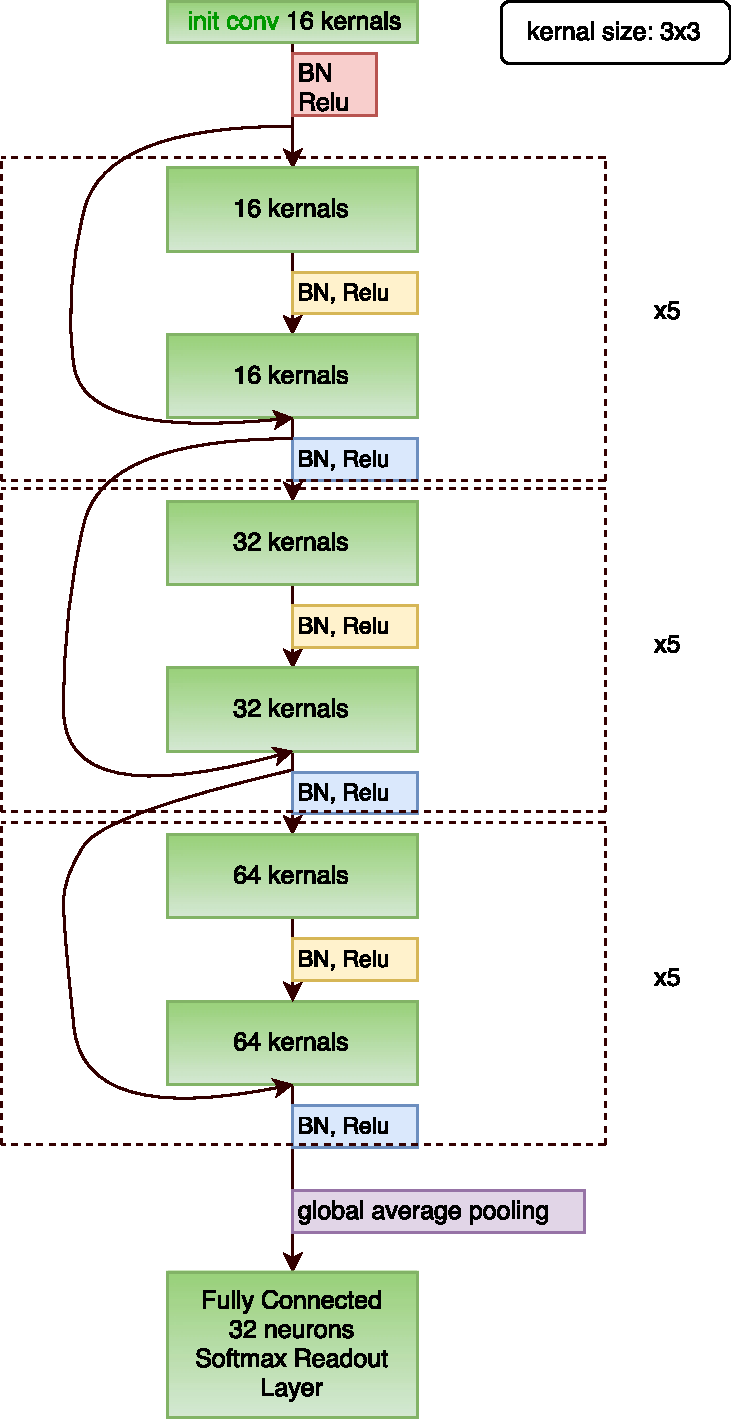
\includegraphics[width=\textwidth,height=\textheight,keepaspectratio]{Figures/our-neural-net-structure.pdf}
    \caption[Neural network architecture for intra mode prediction]{
        Neural network architecture for intra mode prediction.
        }\label{fig:our-architecture}
\end{figure}

\section{Settings of the Network}\label{sec:config}

It is interesting to notice that inside this network, 
the size of any reception field
is always \(3\times3\) since it is found in~\parencite{RN62}
larger kernel can be factorized into smaller kernels.
A kernal with such a size is the smallest
field which is capable of capturing the positional
information~\parencite{RN107}.
All the strides are set to be one which means
no down-sampling will be performed. 
Hence the output size of each convolutional layer
will not be changed.
% The network configuration is shown in Table~\ref{tab:xxxx}.
For the inputs to the convolutional layers, 
zero padding (a.k.a\ SAME padding) is used.
It is a padding algorithm which has the objective
to pad zeros evenly for each direction.
No data augmentation is used for the inputs.
The kernal parameters are randomly initialized 
with a normal distribution where the mean 
is zero while the standard deviation is 
calculated using 
\(\sqrt{2\div(\mathit{a}\times\mathit{a}\times\mathit{n})}\).
Here the \(\mathit{a}\) represents the kernel size
while \(\mathit{n}\) denotes the number of filters
in the corresponding convolutional layer.
The weights of the kernels are regularized by
a decay of \(0.0002\).
No transfer learning is used which means all the learnable 
parameters are trained from scratch.
The batch size used for training is 128.
The loss function used is cross-entropy which has
a better performance for classification problems 
than other distance functions such as L1 and L2.
Stochastic gradient descent is used with a momentum 
of \(0.9\).
The learning rate decay policy is shown in 
Table~\ref{tab:lr-policy}

\begin{table}[H]
    \caption{Learning rate policy}
    \bigskip\label{tab:lr-policy}
    \centering
    \begin{tabular}{c c}
        \toprule
        Global step & Learning rate \\
        \midrule
        \(<\)20,000 & 0.01 \\
        \(<\)40,000 & 0.001 \\
        \(<\)60,000 & 0.0001 \\
        Others  & 0.00001 \\
        \bottomrule
    \end{tabular}
\end{table}
%  0.01 (<20k), 0.001 (<40k), 0.0001 (<60k), 0.00001 (else).


\section{Stopping criteria and Training Results}\label{sec:training}
%Welcome to this \LaTeX{} Thesis Template, a beautiful and easy to use template for writing a thesis using the \LaTeX{} typesetting system.
%
%If you are writing a thesis (or will be in the future) and its subject is technical or mathematical (though it doesn't have to be), then creating it in \LaTeX{} is highly recommended as a way to make sure you can just get down to the essential writing without having to worry over formatting or wasting time arguing with your word processor.
%
%\LaTeX{} is easily able to~\parencite{RN93} professionally typeset documents that run to hundreds or thousands of pages long. With simple mark-up commands, it automatically sets out the table of contents, margins, page headers and footers and keeps the formatting consistent and beautiful. One of its main strengths is the way it can easily typeset mathematics, even \emph{heavy} mathematics. Even if those equations are the most horribly twisted and most difficult mathematical problems that can only be solved on a super-computer, you can at least count on \LaTeX{} to make them look stunning.
%
%%----------------------------------------------------------------------------------------
%
%\section{Welcome and Thanku}\label{sec:welome}
%Welcome to this \LaTeX{} Thesis Template, a beautiful and easy to use template for writing a thesis using the \LaTeX{} typesetting system.
%
%If you are writing a thesis (or will be in the future) and its subject is technical or mathematical (though it doesn't have to be), then creating it in \LaTeX{} is highly recommended as a way to make sure you can just get down to the essential writing without having to worry over formatting or wasting time arguing with your word processor.
%
%\LaTeX{} is easily able to professionally typeset documents that run to hundreds or thousands of pages long. With simple mark-up commands, it automatically sets out the table of contents, margins, page headers and footers and keeps the formatting consistent and beautiful. One of its main strengths is the way it can easily typeset mathematics, even \emph{heavy} mathematics. Even if those equations are the most horribly twisted and most difficult mathematical problems that can only be solved on a super-computer, you can at least count on \LaTeX{} to make them look stunning.
%
%%----------------------------------------------------------------------------------------
%
%\section{Welcome and ThYou}\label{sec:weome}
%Welcome to this \LaTeX{} Thesis Template~\parencite{Reference1}, a beautiful and easy to use template for writing a thesis using the \LaTeX{} typesetting system.
%
%If you are writing a thesis (or will be in the future) and its subject is technical or mathematical (though it doesn't have to be), then creating it in \LaTeX{} is highly recommended as a way to make sure you can just get down to the essential writing without having to worry over formatting or wasting time arguing with your word processor.
%
%\LaTeX{} is easily able to professionally typeset documents that run to hundreds or thousands of pages long. With simple mark-up commands, it automatically sets out the table of contents, margins, page headers and footers and keeps the formatting consistent and beautiful. One of its main strengths is the way it can easily typeset mathematics, even \emph{heavy} mathematics. Even if those equations are the most horribly twisted and most difficult mathematical problems that can only be solved on a super-computer, you can at least count on \LaTeX{} to make them look stunning.
%
%%----------------------------------------------------------------------------------------
%
%\section{Welcome and Thau}\label{sec:welcoe}
%Welcome to this \LaTeX{} Thesis Template, a beautiful and easy to use template for writing a thesis using the \LaTeX{} typesetting system.
%
%If you are
%\begin{table}
%
%    \label{tab:treatments}
%    \centering
%%    \begin{tabular}{l l l}
%%        \toprule
%%        \tabhead{Groups} & \tabhead{Treatment X} & \tabhead{Treatment Y} \\
%%        \midrule
%%        1 & 0.2 & 0.8\\
%%        2 & 0.17 & 0.7\\
%%        3 & 0.24 & 0.75\\
%%        4 & 0.68 & 0.3\\
%%        \bottomrule\\
%%    \end{tabular}
%    \begin{tabular}{c r @{.} l}
%        Pi expression       &
%        \multicolumn{2}{c}{Value} \\
%        \hline
%        $\pi$               & 3&1416  \\
%        $\pi^{\pi}$         & 36&46   \\
%        $(\pi^{\pi})^{\pi}$ & 80662&7 \\
%    \end{tabular}
%    \caption{The effects of treatments X and Y on the four groups studied.}
%\end{table}
%writing a thesis (or will be in the future) and its subject is technical or mathematical (though it doesn't have to be), then creating it in \LaTeX{} is highly recommended as a way to make sure you can just get down to the essential writing without having to worry over formatting or wasting time arguing with your word processor.
%
%\LaTeX{} is easily able to professionally typeset documents that run to hundreds or thousands of pages long. With simple mark-up commands, it automatically sets out the table of contents, margins, page headers and footers and keeps the formatting consistent and beautiful. One of its main strengths is the way it can easily typeset mathematics, even \emph{heavy} mathematics. Even if those equations are the most horribly twisted and most difficult mathematical problems that can only be solved on a super-computer, you can at least count on \LaTeX{} to make them look stunning.
%
%%----------------------------------------------------------------------------------------
%
%\section{Welcome and Tnk You}\label{sec:wlcome}
%Welcome to this \LaTeX{} Thesis Template, a beautiful and easy to use template for writing a thesis using the \LaTeX{} typesetting system.
%
%If you are writing a thesis.
%
%%\begin{verbatim}
%\begin{figure}
%    \centering
%    
\includegraphics{Figures/Electron}
%    %    \decoRule
%    \caption[An Electron]{An electron (artist's impression).}
%    \label{fig:Electron}
%\end{figure}
%%\end{verbatim}
%(or will be in the future) and its subject is technical or mathematical (though it doesn't have to be), then creating it in \LaTeX{} is highly recommended as a way to make sure you can just get down to the essential writing without having to worry over formatting or wasting time arguing with your word processor.
%
%\LaTeX{} is easily able to professionally typeset documents that run to hundreds or thousands of pages long. With simple mark-up commands, it automatically sets out the table of contents, margins, page headers and footers and keeps the formatting consistent and beautiful. One of its main strengths is the way it can easily typeset mathematics, even \emph{heavy} mathematics. Even if those equations are the most horribly twisted and most difficult mathematical problems that can only be solved on a super-computer, you can at least count on \LaTeX{} to make them look stunning.
%
%%----------------------------------------------------------------------------------------